\newpage
\section{Resultados}

\subsection{Simulação do PAM Duobinário}
Os sinais obtidos para a primeira simulação são mostrados na figura 
\ref{fig:ex1}.

\begin{figure}[H]
  \centering
  \caption{Sumilação PAM duobinário.}
  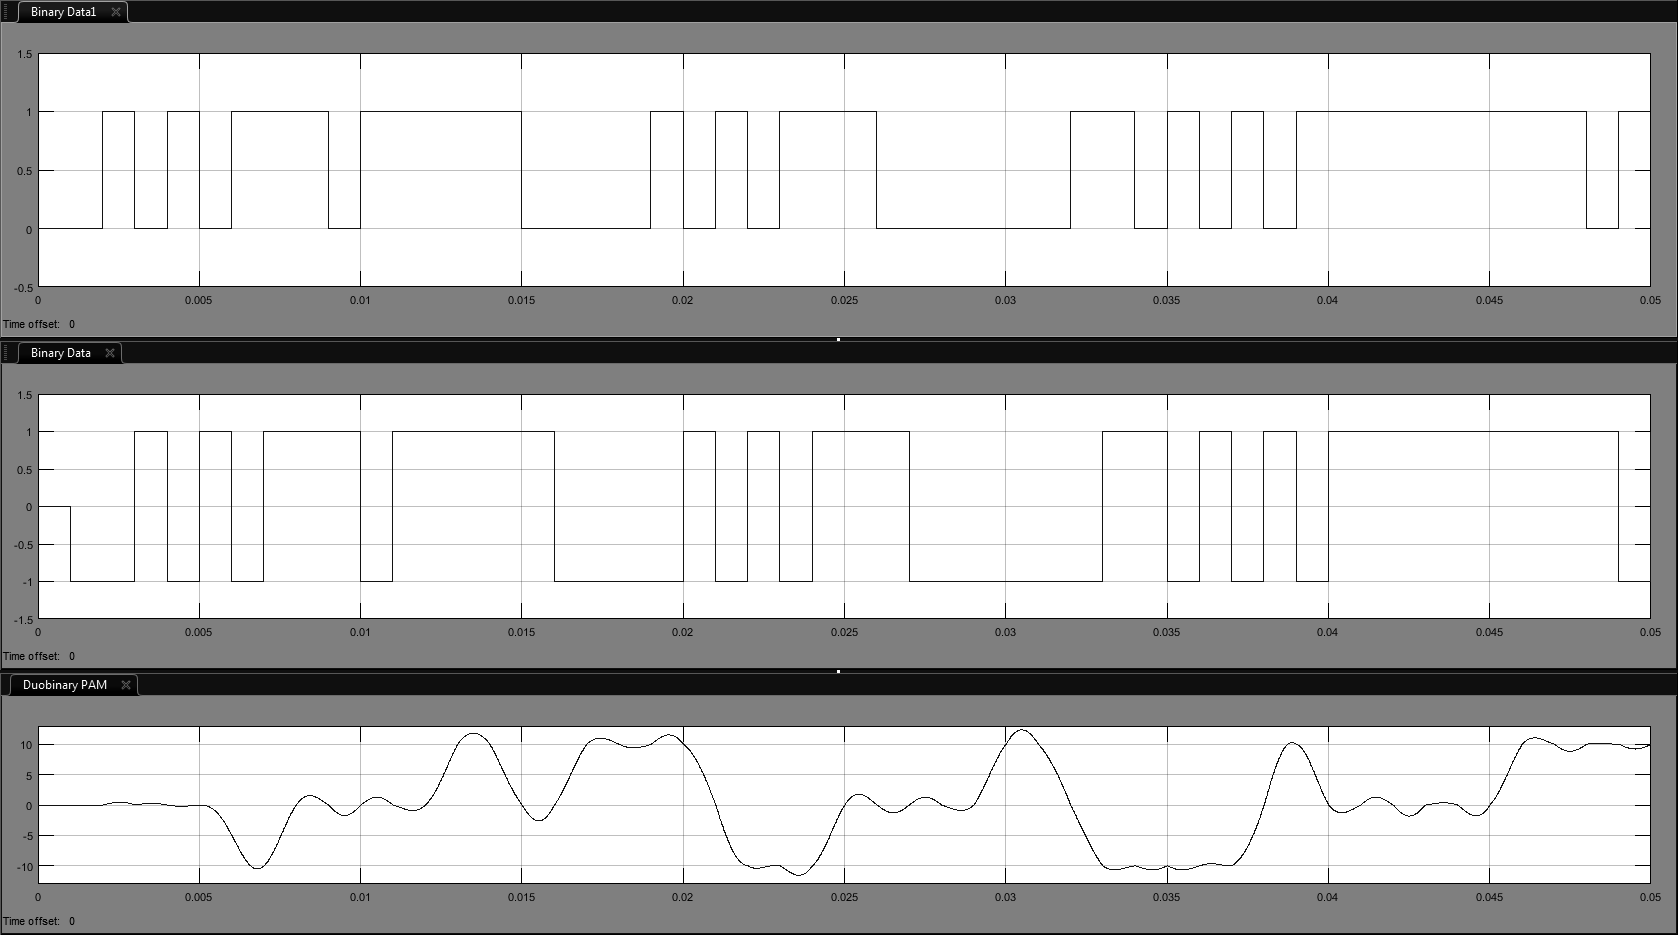
\includegraphics[scale=0.3]{ex1}
  \label{fig:ex1}
\end{figure}

Nota-se que quando a informação fica constante em nível lógico alto, o sinal 
modulado fica positivo e quando a informação fica em nível logico baixo, o 
sinal fica negativo, evidenciando o uso da modulação PAM duobinário.

\subsection{Simulação do PAM Duobinário Modificado}

Os sinais obtidos para a segunda simulação são mostrados na figura  
\ref{fig:ex2}.
\begin{figure}[H]
  \centering
  \caption{Sumilação PAM duobinário modificado.}
  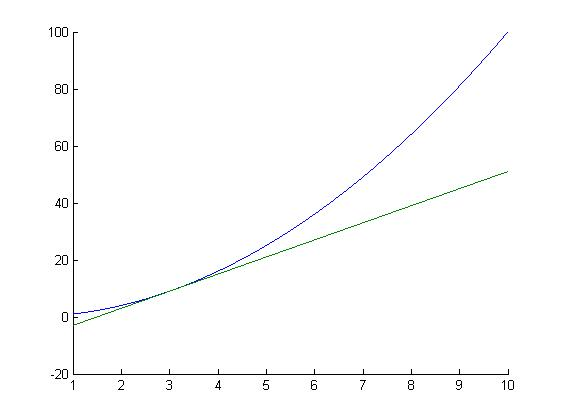
\includegraphics[scale=0.3]{ex2}
  \label{fig:ex2}
\end{figure}

Aqui é mais difícil ver a modulação, devido ao fato que o duobinário modificado 
utiliza um bit com atraso para modular o sinal.

\subsection{Desempenho para o PAM Duobinário em um Receptor Simples no Canal 
AWGN}

Os sinais obtidos para a terceira simulação são mostrados na figura  
\ref{fig:ex3}.
\begin{figure}[H]
  \centering
  \caption{Sumilação PAM duobinário com canal AWGN.}
  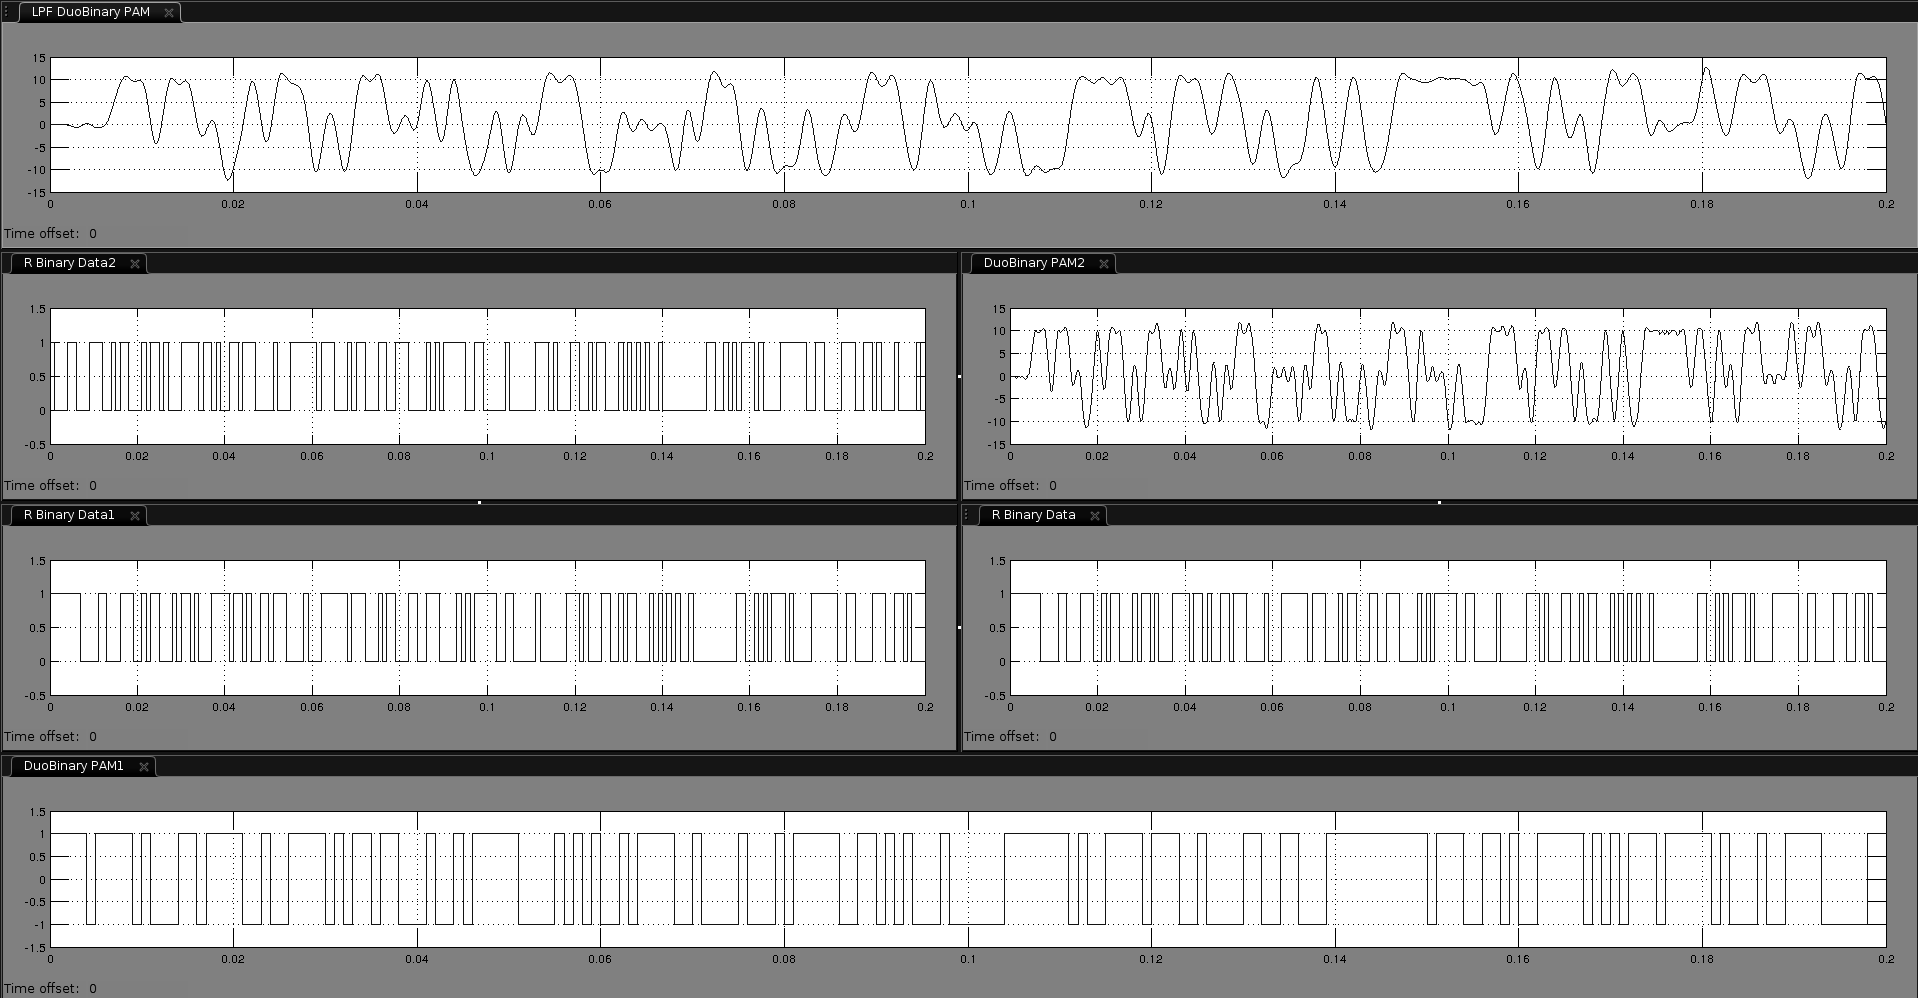
\includegraphics[scale=0.3]{ex3}
  \label{fig:ex3}
\end{figure}
        
 A tabela \ref{tab:ex3} mostra os valores obtidos com as simulações.
 
\begin{table}[H]
  \begin{center}
    \caption{Tabela BER x Eb/No para PAM duobinário.}
    \begin{tabular}{|c|c|c|}
      \hline
      SNR (dB) & AWGN $\sigma^2 (V^2)$ & BER \\
      \hline
      7.04 & 10 & 0 \\
      \hline
      2.05 & 50 &  0.0015\\
      \hline
      -6.8122 & 100 & 0.0035\\
      \hline
      -13.7437 & 200 & 0.0238 \\
      \hline
      -17.7983 & 300 & 0.0549  \\
      \hline
      -20.6751 & 400 & 0.0888 \\
      \hline 
      -22.9066 & 500 & 0.1247\\
      \hline
    \end{tabular}
    \label{tab:ex3}
  \end{center}
\end{table}

\subsection{Desempenho para o PAM Duobinário Modificado em um Receptor 
Simples no Canal AWGN}

Os sinais obtidos para a quarta simulação são mostrados na figura  
\ref{fig:ex4}.
\begin{figure}[H]
  \centering
  \caption{Sumilação PAM duobinário modificado com canal AWGN.}
  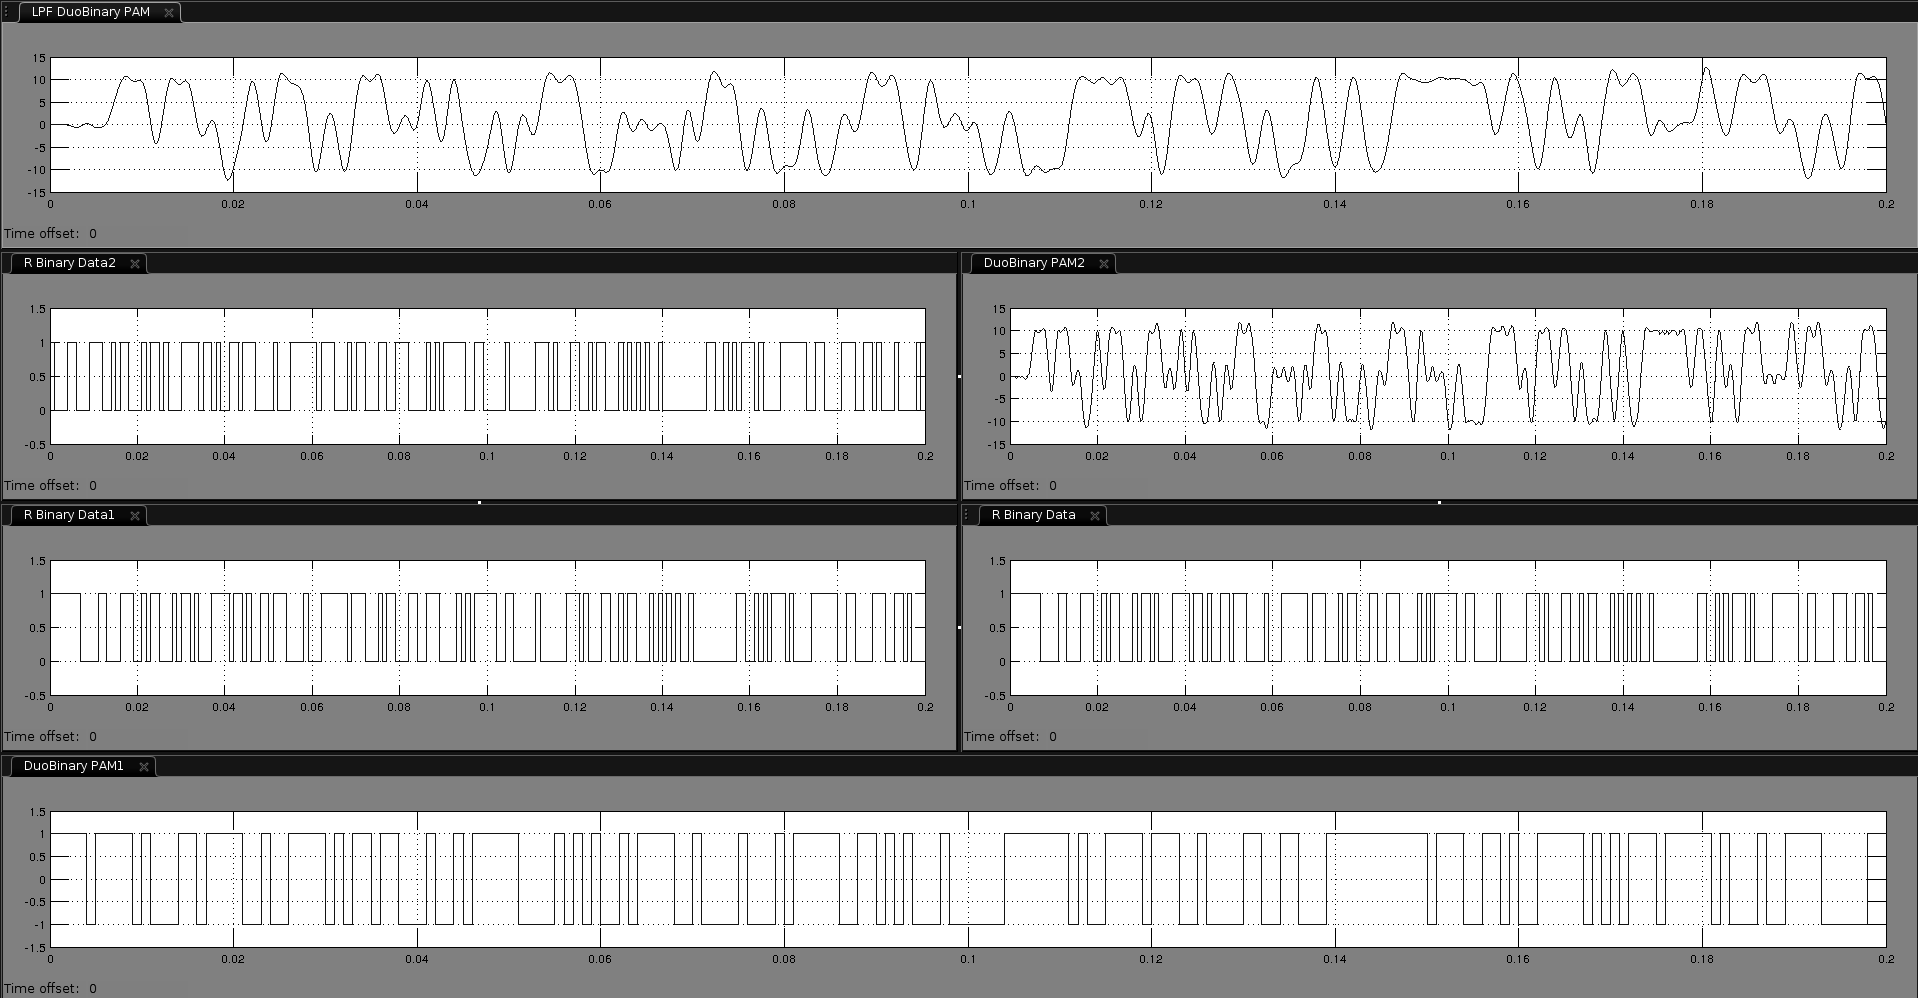
\includegraphics[scale=0.3]{ex3}
  \label{fig:ex4}
\end{figure}

              
 
\begin{table}[H]
  \begin{center}
    \caption{Tabela BER x Eb/No para PAM duobinário modificado.}
    \begin{tabular}{|c|c|c|}
      \hline
      SNR (dB) & AWGN $\sigma^2 (V^2)$ & BER \\
      \hline
      7.01 & 10 & 0 \\
      \hline
      2.02& 50 & 0 \\
      \hline
      -6.8916 & 100 & 0.0053\\
      \hline
     -13.8230& 200 & 0.0309\\
      \hline
      -17.8777& 300 & 0.0638\\
      \hline
      -20.7545& 400 & 0.1019\\
      \hline 
      -22.9859& 500 & 0.1278\\
      \hline
    \end{tabular}
    \label{tab:simmdb}
  \end{center}
\end{table}

A figura \ref{fig:ex4b} mostra uma comparação entre os dois sistemas, nota-se 
que o sistema duobinário simples é melhor.
\begin{figure}[H]
  \centering
  \caption{Comparação PAM duobinário com PAM duobinário modificado com canal 
  AWGN.}
  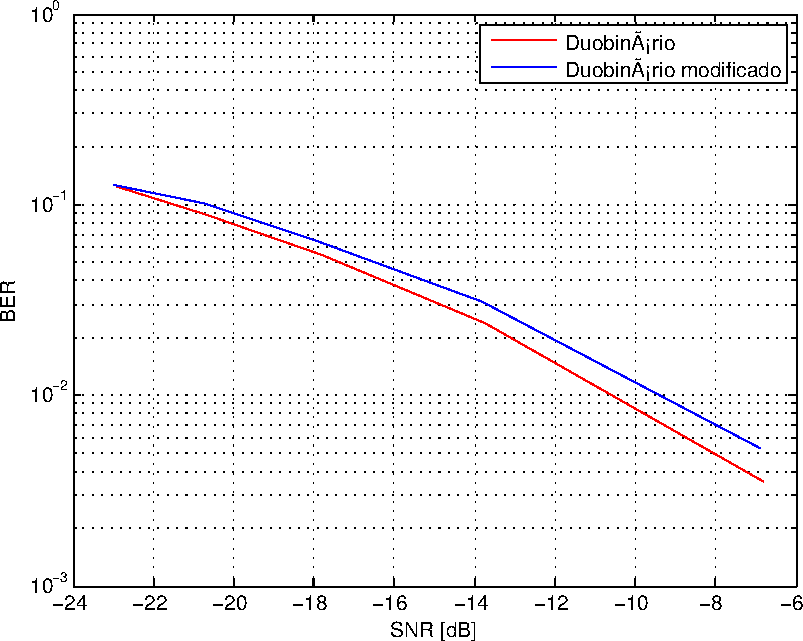
\includegraphics[scale=1]{ex4b}
  \label{fig:ex4b}
\end{figure}

\subsubsection{Densidade Espectral de Potência (PSD) dos PAM Duobinários}
 As figura \ref{fig:ex5a} e \ref{fig:ex5b} mostram a densidade espectral de 
 potência para os sistemas com sinalização duobinário e duobinário modificado, 
 respectivamente.
 
 Nota-se a redução na PSD para frequências próximas de 0Hz no sistema 
 duobinário modificado.
 
\begin{figure}[H]
  \centering
  \caption{PSD PAM duobinários.}
  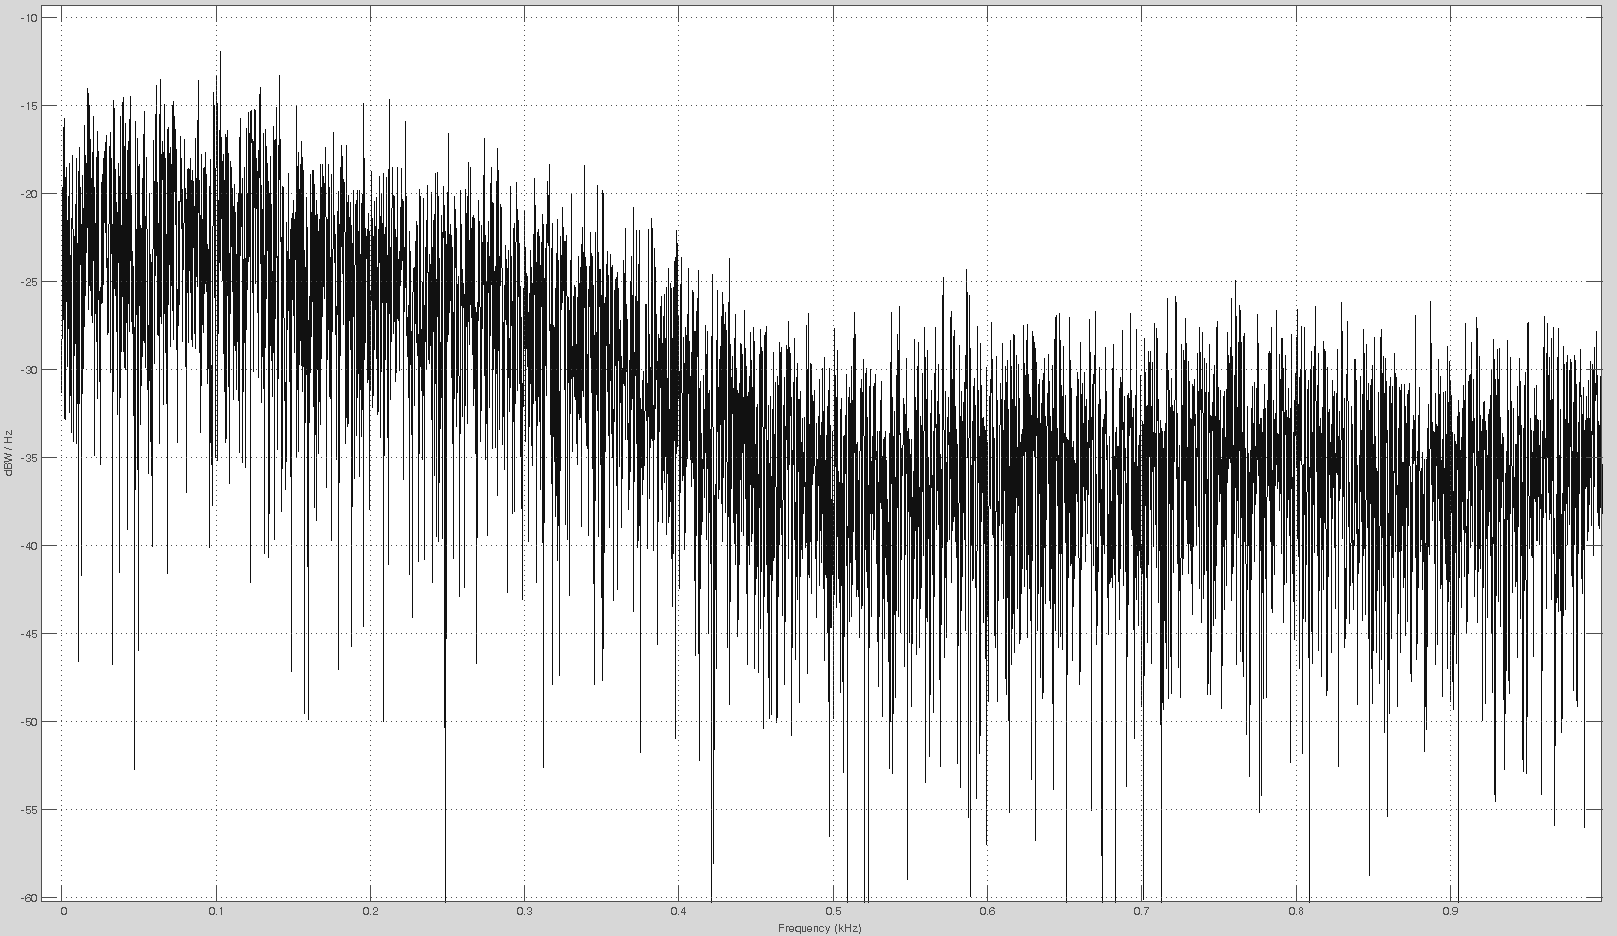
\includegraphics[scale=0.2]{ex5a}
  \label{fig:ex5a}
\end{figure}

\ref{fig:ex5b}.
\begin{figure}[H]
  \centering
  \caption{PSD PAM duobinários modificado.}
  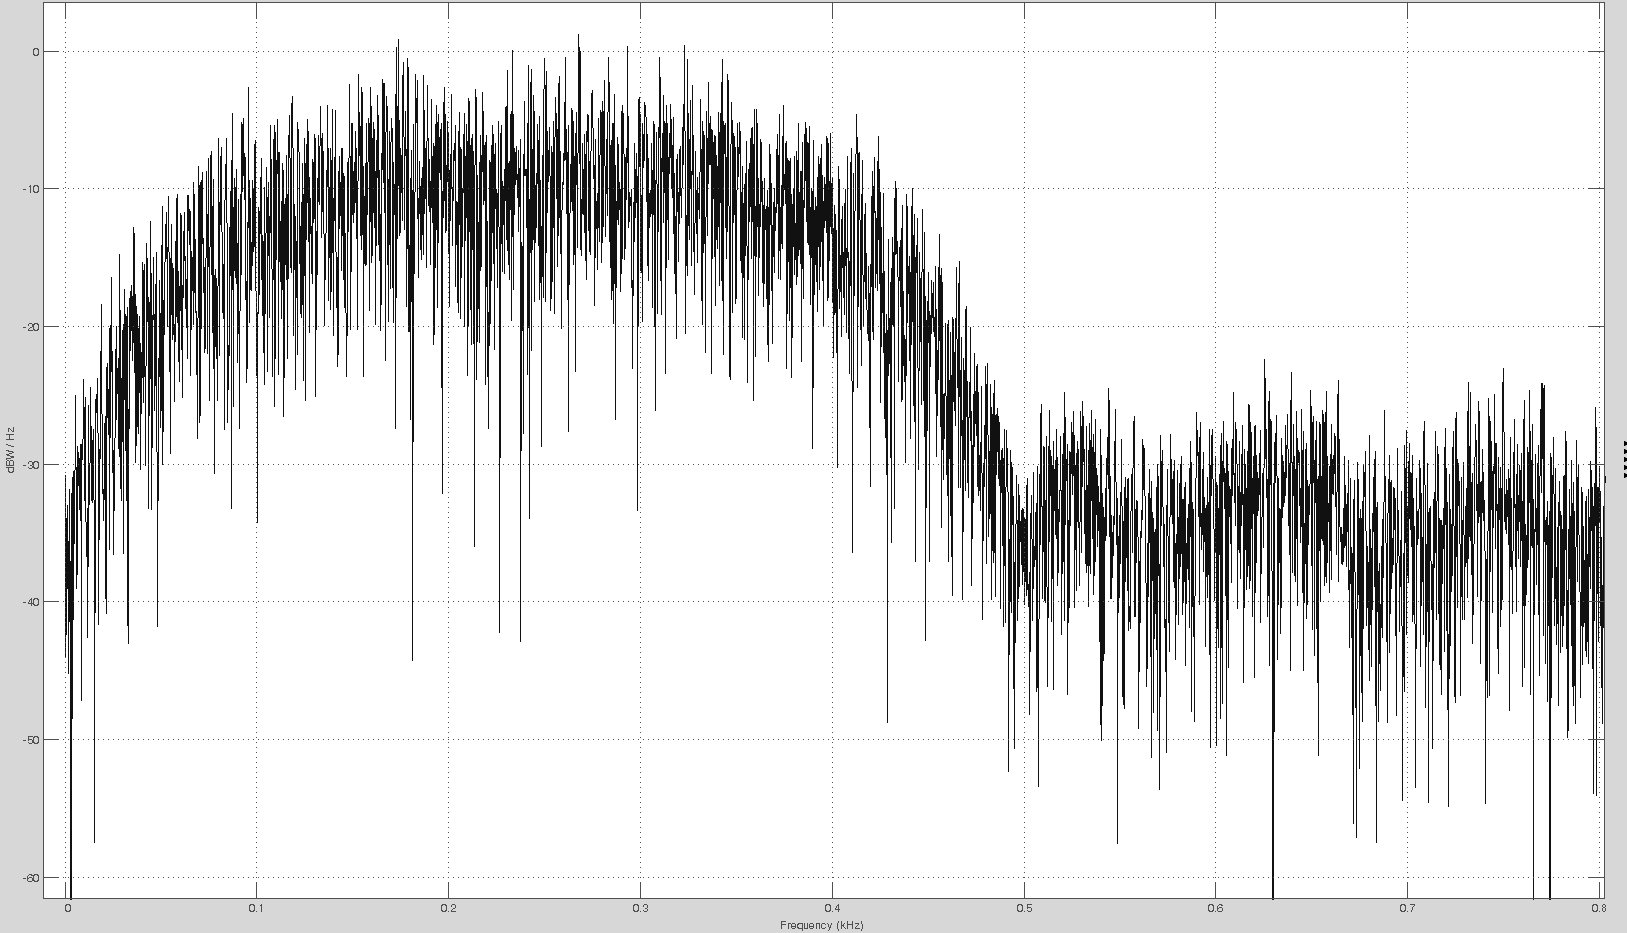
\includegraphics[scale=0.2]{ex5b}
  \label{fig:ex5b}
\end{figure}